\documentclass[12pt,a4paper]{article}

\usepackage[UTF8]{ctex}
\usepackage{amsmath,amscd,amsbsy,amssymb,latexsym,url,bm,amsthm}
\usepackage{amsfonts}
\usepackage{epsfig,graphicx,subfigure}
\usepackage{hyperref}
\usepackage{listings}
\usepackage[vlined,ruled,linesnumbered]{algorithm2e}
\usepackage{enumitem}
\usepackage{xcolor}
\usepackage{geometry}

%\uppercase\expandafter{\romannumeral1}:% 罗马数字。

\lstset{
language=Matlab,
keywordstyle= \color{blue!70},
commentstyle= \color{red!50!green!50!blue!50},
breaklines
}%设置listing插入语言

\setlength{\parindent}{0em}
\setlength{\parskip}{1em}

\geometry{bottom =3cm}
\newcommand{\textbi}[1]{%
\textbf{\textit{#1}}}

\newcommand{\ncolor}[1]{%
{\color[RGB]{139,117,0}{#1}}}
\newtheorem{theorem}{Theorem}[section]
\newenvironment{solution}{{\noindent \it \textbf{Solution:}}\\}

\title{MCM daily}
\author{Yunlong Cheng}

\begin{document}
\maketitle
\section{2018-B题-智能RGV动态调度简述}
总共有8台数控机床(CNC), 1辆轨道式自动引导车(RGV), 1条上料带、1条下料带。RGV小车负责“上料,清洗,下料”。

\begin{center}
  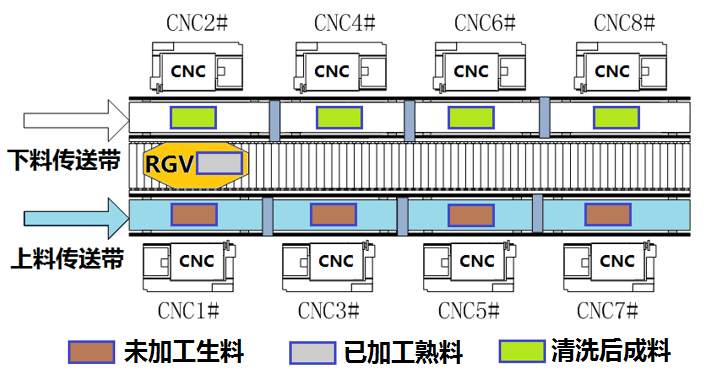
\includegraphics[width = 0.9\textwidth]{figures/illustrate-diagram.png}
\end{center}
针对以下三种情况完成两项任务:
\begin{itemize}
  \item 一道工序的物料加工,物料可以在任一台 CNC 加工。
  \item 两道工序的加工,物料的两道工序分别由不同的 CNC 完成。
  \item CNC 加工可能出现故障,故障排除需要人工完成
\end{itemize}
任务:
\begin{itemize}
  \item 对于一般问题给出 RGV 调度模型和算法。
  \item 利用参数检验模型实用性和算法的有效性,给出RGV调度策略和系统作业效率,并将具体结果填入附件2。
\end{itemize}

\section{分析}
\subsection{任务1}
\subsubsection{无故障下的一道工序}
\begin{table}[!htbp]
  \caption{符号定义}
  \centering
  \begin{tabular}{c|c}
    \hline
    Z& 总完成工件\\
    $x_i^{(k)}$& 第k轮上料 RGV 是否前往第 i 个机器\\
    $T_i^{(k)}$& RGV 前往第 i 台CNC并上料的时间\\
    $f_i^{(k)}$& 第i台CNC是否有物料\\
    \hline
  \end{tabular}
\end{table}
其中决策变量为$x_i^{(k)}$。所以模型:
\begin{equation*}
  \begin{split}
    maximize\quad Z&\\
    subject\; to&\\
    T_i^{(k)} & = min_iT_i^{(k)}\\
    T_i^{(k)} & = max_i(T_{sheni}^{(k)}, T_{yip^{(k)}q^{(k)}}^{(k)})\\
    \sum_{i = 1}^8x_i^{(k)} & = 1\\
    f_i^{(k+1)} & = f_i^{(k)} + x_i^{(k)}(1-f_i^{(k)})\\
    \sum_{k = 1}^k\sum_{i = 1}^8x_i^{(k)}(T_i^{(k)} + T_{xii}^{(k)}\cdot f_i^{(k)})& \le 8\times 3600\\
  \end{split}
\end{equation*}
\textbf{解决算法:}
贪心为主,每一次RGV小车都选择移动和上料时间最快的CNC进行作业。

\subsubsection{无故障下的两道工序}
\begin{table}[!htbp]
  \caption{符号定义}
  \centering
  \begin{tabular}{c|c}
    \hline
    $X^{(k)}$ & 物料加工状态\\
    $Y_i$ & 刀具加工工序\\
    \hline
  \end{tabular}
\end{table}
对应的\textbf{约束条件}也要增加:
\begin{equation*}
  Y_i =
  \begin{cases}
    1 & $第 i 台 CNC 负责第一道工序$\\
    2 & $第 i 台 CNC 负责第二道工序$
  \end{cases}
\end{equation*}
\begin{equation*}
  X^{(k)} =
  \begin{cases}
    1 & $第 k 轮上料时 RGV 内无物料$\\
    2 & $第 k 轮上料时 RGV 有工序一物料$
  \end{cases}
\end{equation*}
$$x_i^{(k)} = x_i^{(k)}(1-|x_i^{(k)}-Y_i|)$$
$$a + b = 8;a,b \in N^+$$

因为两种刀具至少要有一个,所以共有$\sum_{i = 1}^7C_8^j = 254$种刀具分配方法,遍历每种分配方法得出最优刀具分配。

\textbf{求解算法}:
RGV 找到能最快完成上下料的 CNC,并响应此 CNC 的当轮需求信号,再根据实际情况判断是否洗料记忆是否改变目标工序。

\subsubsection{故障下的一道工序情况}
\begin{table}[!htbp]
  \caption{新增符号定义}
  \centering
  \begin{tabular}{c|c}
    \hline
    $T_{\text{渡}i}^{(k)}$ & 机器工作后到发生故障的过渡时间\\
    $T_{\text{修}i}^{(k)}$ & CNC 修理时间\\
    \hline
  \end{tabular}
\end{table}

新增约束条件:
\begin{equation*}
T_{\text{渡}i}^{(k)} \sim U(0,T_{工i}^{(k)})
\end{equation*}
\begin{equation*}
  P(C_i^{(k)}) = \frac{1}{100}
\end{equation*}
$$T_{\text{修}i}^{(k)} \sim U(600,1200)$$
并且 $$f_i^{(k+1)} = 0,T_{\text{剩}i}^{(k)} = T_{\text{修}i}^{(k)}$$

\textbf{求解算法:}
通过随机数模拟故障和维修,将故障时间转化为工作时间。算法与无故障下的一道工具类似,核心思路也是 Greedy。

\subsubsection{故障下的两道工序情况}
将原有约束结合一道工序的约束构成此约束,无新增约束。

\textbf{求解方法:}
与无故障两道工序算法类似。

\subsection{任务二}
利用所给三组参数检验模型实用性和算法有效性。
\subsubsection{模型实用性}
\begin{itemize}
  \item 实施的可能性
  \item 经济性
  \item 普适性
  \item CNC 平均非有效工作时长
\end{itemize}
\subsubsection{算法有效性}
\begin{itemize}
  \item 程序运行总时长
  \item 程序运行占用内存
\end{itemize}

\section{模型检验和灵敏度分析}
优缺点,改进,推广与运用
\section{参考文献}
\section{Code}
\end{document}
